\section{Lista 4: Método dos Mínimos Quadrados} % <-----------------------------------------------------------------------------

\subsection{Algoritmo RLS} % <-----------------------------------------------------------------------------
As tabelas~\ref{tab:fixcoef} e \ref{tab:freecoef} apresentas as 10 primeiras iterações dos coeficientes de filtro, para caso $w_0$ seja fixo igual a um ou possa atualizar livremente. É possível observar que a oscilação fica cada menor ao se aproximar da 10ª iteração.

\begin{table}[!htp]
    \centering
    \begin{tabular}{ l l l l }
        \hline
        Iterations & $w_{0}$ & $w_{1}$ & $w_{2}$ \\ 
        \hline 
        1 & 1 & 0 & 0 \\ \hline
        2 & - & -0.0161 & -0.0130 \\ \hline
        3 & - & -0.0168 & -0.0472 \\ \hline
        4 & - & 0.0048 & -0.0518 \\ \hline
        5 & - & 0.0320 & -0.0831 \\ \hline
        6 & - & 0.0504 & -0.0561 \\ \hline
        7 & - & -0.0231 & 0.0466 \\ \hline
        8 & - & 0.0630 & 0.1069 \\ \hline
        9 & - & 0.0568 & 0.1192 \\ \hline
        10 & - & 0.0796 & 0.1457 \\ \hline
    \end{tabular}
    \caption{Atualização do filtro com o $w_0$ fixo igual a um.}
    \label{tab:fixcoef}
\end{table}

\begin{table}[!htp]
    \centering
    \begin{tabular}{l l l l}
        \hline
        Iterations & $w_{0}$ & $w_{1}$ & $w_{2}$ \\ 
        \hline \hline
        1 & 1 & 0 & 0 \\ \hline
        2 & 0.9860 & -0.0161 & -0.0130 \\ \hline
        3 & 0.9611 & -0.0167 & -0.0435 \\ \hline
        4 & 0.9687 & 0.0134 & -0.0499 \\ \hline
        5 & 0.9322 & 0.0369 & -0.0769 \\ \hline
        6 & 0.9053 & 0.0609 & -0.0419 \\ \hline
        7 & 0.8471 & 0.0034 & 0.0384 \\ \hline
        8 & 0.7149 & 0.0642 & 0.0809 \\ \hline
        9 & 0.7264 & 0.0767 & 0.0558 \\ \hline
        10 & 0.7125 & 0.0843 & 0.0646 \\ \hline
    \end{tabular}
    \caption{Atualização do filtro com o $w_0$ livre para atualizar.}
    \label{tab:freecoef}
\end{table}

A título de comparação, foi implementado ambos os casos de atualização do coeficientes $w_0$. A Figura~\ref{fig:hw4p1} mostra os sinais obtidos com ambos os vetores de filtro, que se aproximam consideravelmente do sinal original, senoidal entre $(-3\pi,3\pi)$.

Na inicialização do filtro, ambos distam igualmente do sinal desejado, porém ao passo que mais amostras são utilizadas no processo de adaptação, ambos se aproximam do sinal alvo. Apresentando maiores oscilações justamente nos pontos inflexão, dado a variação mais abrupta.

É possível observar também que o algoritmo com livre adaptação para $w_0$ apresenta desempenho melhor que o proposto, dado que existe um coeficiente a mais para garantir que a adaptação será mais adequada que ao manter um valor fixo e atualizar apenas dois coeficientes.

\clearpage

\begin{figure}[!htp]
    \centering
    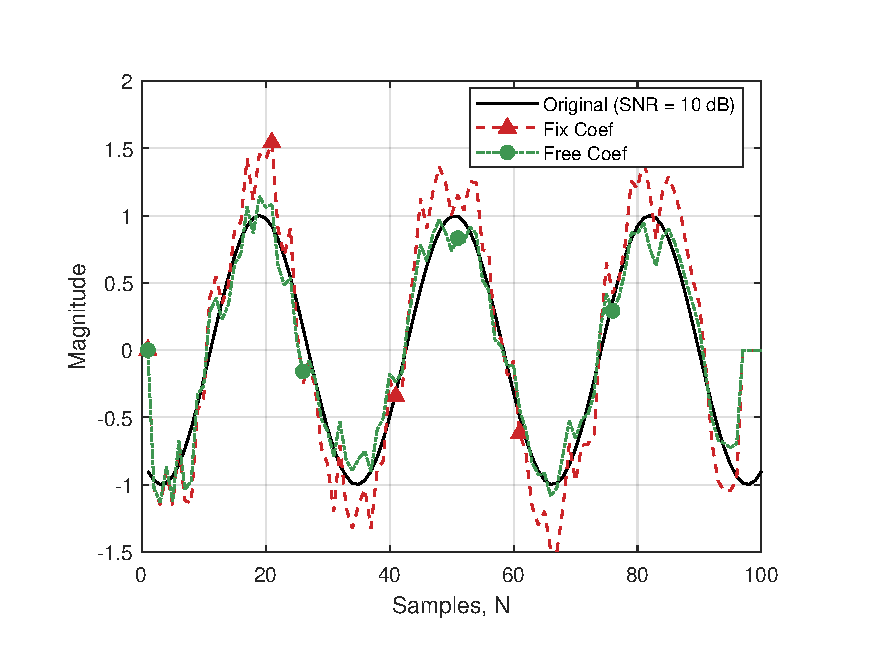
\includegraphics[width=1.0\textwidth]{C:/Users/lucasabdalah-dell/Documents/GitHub/Courses-HWs/Master/TIP7188-FILTRAGEM_ADAPTATIVA/homework/code/figures/hw4p1.pdf}
    \caption{Primeiro coeficiente livre para adaptação com $\text{Amostras} = 100$, $M = 2$, $\lambda = 0.98$}
    \label{fig:hw4p1}
\end{figure}


% \subsection{Erro de Estimação a Priori} % <-----------------------------------------------------------------------------
% \todo[inline, color=yellow!30]{Organizar}
    
% \begin{align}
%     \epsilon(n) = d(n) - \boldsymbol{w}^{\text{H}}(n - 1) \boldsymbol{x}(n),
% \end{align}

% em que $d(n)$ é a resposta desejada, $x(n)$ é o vetor de entrada do filtro e $\boldsymbol{w}(n - 1)$ é a estimativa
% anterior do vetor de coeficientes do filtro. Seja $e(n)$ o erro de estimação a posteriori

% \begin{align}
%     e(n) = d(n) - \boldsymbol{w}^{\text{H}}(n) \boldsymbol{x}(n),
% \end{align}

% em que $\boldsymbol{w}(n)$ é a estimativa atual do vetor de coeficientes do filtro. Para dados complexos ambos
% $\epsilon(n)$ e $e(n)$ são de valores complexos. Mostre que o produto $\epsilon(n)e^{*}(n)$ é sempre de valor real.

% \textcolor{red}{Solução:}

% Primeiramente é necessário reescrever $e(n)$ em termos de $\epsilon(n)$. Inicialmente podemos escrever os coeficientes de filtro do instante $n$,
% utilizando o erro a priori, da seguinte forma

% \begin{align}
%     \boldsymbol{w}(n) = \boldsymbol{w}(n-1) + \epsilon(n) \boldsymbol{S}_{D}(n) \boldsymbol{x}(n),
% \end{align}

% e em seguida substituímos a expressão acima na definição do erro de estimação instantâneo e obtemos 

% \begin{align}
%     e(n) &= d(n) - \boldsymbol{w}^{\text{H}}(n) \boldsymbol{x}(n), \\
%     e(n) &= d(n) - \boldsymbol{x}^{\text{H}}(n) \boldsymbol{w}(n), \\
%     e(n) &= d(n) - \boldsymbol{x}^{\text{H}}(n) \left[\boldsymbol{w}(n-1) + \epsilon(n) \boldsymbol{S}_{D}(n) \boldsymbol{x}(n)\right], \\
%     e(n) &= d(n) - \boldsymbol{x}^{\text{H}}(n) \boldsymbol{w}(n-1) - \boldsymbol{x}^{\text{H}}(n) \epsilon(n) \boldsymbol{S}_{D}(n) \boldsymbol{x}(n), \\
%     e(n) &= \underbrace{d(n) - \boldsymbol{x}^{\text{H}}(n) \boldsymbol{w}(n-1)}_{\epsilon(n)} - \epsilon(n) \boldsymbol{x}^{\text{H}}(n) \boldsymbol{S}_{D}(n) \boldsymbol{x}(n), \\
%     e(n) &= \epsilon(n) - \epsilon(n) \boldsymbol{x}^{\text{H}}(n) \boldsymbol{S}_{D}(n) \boldsymbol{x}(n), \\
% \end{align}

% e em sequência desenvolvemos o conjugado de $e(n)$ do seguinte modo

% \begin{align}
%     e^{*}(n) &= \epsilon^{*}(n) - \epsilon^{*}(n) \boldsymbol{x}^{\text{H}}(n) \boldsymbol{S}_{D}(n) \boldsymbol{x}(n),
% \end{align}

% onde o termo $\boldsymbol{x}^{\text{H}}(n) \boldsymbol{S}_{D}(n) \boldsymbol{x}(n)$ é a distância de Mahalanobis que será sempre real e positiva.
% Desse modo, ao fazermos $\epsilon(n) e^{*}(n)$ obtemos 

% \begin{align}
%     \epsilon(n) e^{*}(n) &= \epsilon(n) \left[\epsilon^{*}(n) - \epsilon^{*}(n) \boldsymbol{x}^{\text{H}}(n) \boldsymbol{S}_{D}(n) \boldsymbol{x}(n)\right], \\
%     \epsilon(n) e^{*}(n) &= \epsilon(n) \epsilon^{*}(n) - \epsilon(n) \epsilon^{*}(n) \boldsymbol{x}^{\text{H}}(n) \boldsymbol{S}_{D}(n) \boldsymbol{x}(n), \\
%     \epsilon(n) e^{*}(n) &= \epsilon(n) \epsilon^{*}(n) \left(1 - \boldsymbol{x}^{\text{H}}(n) \boldsymbol{S}_{D}(n) \boldsymbol{x}(n)\right).
% \end{align}

% Dessa forma, sabemos que o termos $\left(1 - \boldsymbol{x}^{\text{H}}(n) \boldsymbol{S}_{D}(n) \boldsymbol{x}(n)\right)$ será sempre real, embora nem sempre positivo,
% e $\epsilon(n) \epsilon^{*}(n)$ pode simplesmente ser visto como uma norma dada por $||\epsilon(n)||^{2} = \epsilon(n) \epsilon^{*}(n)$, demonstrando assim que sempre 
% teremos um valor real para $\epsilon(n) e^{*}(n)$.


% \subsection{Preditor Adaptativo} % <-----------------------------------------------------------------------------
% \todo[inline, color=yellow!30]{Organizar}
% Os resultados podem ser encontrados nas Figuras \ref{fig:L4Q3_a1} - \ref{fig:L4Q3_a8}. Nas figuras \ref{fig:L4Q3_a1} e \ref{fig:L4Q3_a2} temos a evolução
% dos coeficientes de filtro e do MSE para o RLS com fator de esquecimento $\lambda = 0.9$, SNR = $3$ dB e ordens $M = 2$ e $M = 3$, respectivamente. Nesses cenários podemos 
% ver que o RLS não atingiu a estabilidade em seus coeficientes de filtro embora tenha apresentado um comportamento MSE sem grandes variâncões de magnitude. Ademais, no segundo cenário
% é possível verificar maior estabilidade na evolução do MSE graças ao incremento na ordem do RLS. Em sequência, nas Figuras \ref{fig:L4Q3_a3} e \ref{fig:L4Q3_a4} temos dois cenárioss similares, 
% mas agora com um fator dde conhecimento igual a $\lambda = 0.99$. Diferentemente dos dois primeiros cenários agora é possível verificar que o RLS atingiu estabilidade em seus coeficientes de filtro, 
% além de um melhor desempenho na evolução do MSE do que nos casos anteriores. Isso se deve pois, diferente do que ocorre com o passo de aprendizado nos algoritmos estudados anteriormente, a medida que
% $\lambda$ cresce menos fléxivel torna-se o filtro. Desse modo, é mais fácil para esses novos cenários adaptem-se à evolução do canal com maior facilidade. Alem disso, novamente foi possível observar 
% o impacto da ordem do RLS na estabilidade da evolução do MSE, onde para o cenário $M = 3$ foi verificado um melhor desempenho do que para o cenário $M = 2$.

% Por fim, nos resta analisar o impacto da SNR na estabilidade e desempenho do RLS. Nas Figuras \ref{fig:L4Q3_a5} e \ref{fig:L4Q3_a6} temos o equivalente ao primeiro par de cenários, mas agora 
% com a diferença de que ambos os cenários são de SNR infinita. Para o primeiro caso com $M = 2$ vemos uma estabilização perfeita dos coeficientes do filtro e uma evolução do erro MSE que tende ao erro de
% precisão da máquina. Dessa forma, podemos considerar esse um cenário ideal para o RLS. Sequencialmente, na figura seguinte consideramos um cenário $M = 3$ e podemos verificar que não existiu convergência para
% esse cenário. Inicialmente existiu uma certa estabilização na evolução do MSE, mas apos algumas iterações o filtro perdeu a estabilidade e seus coeficientes "explodiram". Esse comportamento pode ser explicado 
% tanto pelo aumento da ordem do filtro quanto pelo fator de esquecimento que torna o filtro muito pouco fléxivel e suscetível a instabilidades provocadas por mudanças repentinas. Por fim, nas Figuras \ref{fig:L4Q3_a7}
% e \ref{fig:L4Q3_a8} temos dois resultados estáveis na evolução do MSE e nos coeficientes do filtro RLS. Isso se deve principalmente a um fator de esquecimento que fornece maior capacidade de resistir a instabilidades
% geradas pelo canal.

% \begin{figure}[!htp]
%     \centering
%     %\includegraphics[width=0.825\textwidth]{figs/L4Q3_rls_mse_2_3_9.png}
%     \includegraphics[width=0.5\textwidth]{example-image}
%     \caption{SNR = 3 dB, M = 2 and $\lambda = 0.9$}
%     \label{fig:L4Q3_a1}
% \end{figure}

% \begin{figure}[!htp]
%     \centering
%     %\includegraphics[width=0.825\textwidth]{figs/L4Q3_rls_mse_3_3_9.png}
%     \includegraphics[width=0.5\textwidth]{example-image}
%     \caption{SNR = 3 dB, M = 3 and $\lambda = 0.9$}
%     \label{fig:L4Q3_a2}
% \end{figure}

% \begin{figure}[!htp]
%     \centering
%     %\includegraphics[width=0.825\textwidth]{figs/L4Q3_rls_mse_2_3_99.png}
%     \includegraphics[width=0.5\textwidth]{example-image}
%     \caption{SNR = 3 dB, M = 2 and $\lambda = 0.99$}
%     \label{fig:L4Q3_a3}
% \end{figure}

% \begin{figure}[!htp]
%     \centering
%     %\includegraphics[width=0.825\textwidth]{figs/L4Q3_rls_mse_3_3_99.png}
%     \includegraphics[width=0.5\textwidth]{example-image}
%     \caption{SNR = 3 dB, M = 3 and $\lambda = 0.99$}
%     \label{fig:L4Q3_a4}
% \end{figure}

% \begin{figure}[!htp]
%     \centering
%     %\includegraphics[width=0.825\textwidth]{figs/L4Q3_rls_mse_2_inf_9.png}
%     \includegraphics[width=0.5\textwidth]{example-image}
%     \caption{SNR = $\infty$ dB, M = 2 and $\lambda = 0.9$}
%     \label{fig:L4Q3_a5}
% \end{figure}

% \begin{figure}[!htp]
%     \centering
%     %\includegraphics[width=0.825\textwidth]{figs/L4Q3_rls_mse_3_inf_9.png}
%     \includegraphics[width=0.5\textwidth]{example-image}
%     \caption{SNR = $\infty$ dB, M = 3 and $\lambda = 0.9$}
%     \label{fig:L4Q3_a6}
% \end{figure}

% \begin{figure}[!htp]
%     \centering
%     %\includegraphics[width=0.825\textwidth]{figs/L4Q3_rls_mse_2_inf_99.png}
%     \includegraphics[width=0.5\textwidth]{example-image}
%     \caption{SNR = $\infty$ dB, M = 2 and $\lambda = 0.99$}
%     \label{fig:L4Q3_a7}
% \end{figure}

% \begin{figure}[!htp]
%     \centering
%     % \includegraphics[width=0.825\textwidth]{figs/L4Q3_rls_mse_3_inf_99.png}
%     \includegraphics[width=0.5\textwidth]{example-image}
%     \caption{SNR = $\infty$ dB, M = 3 and $\lambda = 0.99$}
%     \label{fig:L4Q3_a8}
% \end{figure}
% \clearpage


% \subsection{Equalização de Canais} % <-----------------------------------------------------------------------------
% \todo[inline, color=red!30]{Finalizar}
% % \begin{enumerate}
    
% %     \item Calcule a adaptação do algoritmo usando o RLS e mostre a evolução temporal dos coeficientes.

% %         \textcolor{red}{Solução:}

% %         A evolução temporal dos coeficientes do filtro pode ser encontrada na Figura \ref{fig:rls_coefficient}.  
% %         Aqui é possível verificar a convergência e estabilização dos coeficientes do filtro partindo do zero a medida que o número 
% %         de iterações cresce. Existem algumas oscilações ao final do processo, mas nada considerável. Caso o fator de esquecimento fosse
% %         aumentado possivelmente haveriam oscilações com maiores magnitudes nos coeficientes de filtro. 

% %     \item Obtenha as trajetórias sobre as curvas de nível, tendo condições iniciais nulas para os
% %     coeficientes do equalizador. Verifique qual a melhor inicialização do algoritmo RLS. Compare
% %     com os algoritmos LMS, LMS-Normalizado e Gauss-Newton.

% %         \textcolor{red}{Solução:}

% %         As trajetórias dos algoritmos Newton, Gradiente, LMS e NLMS estão disponíveis nas Figuras \ref{fig:newton_contour}, \ref{fig:gradient_contour}, 
% %         \ref{fig:lms_contour} e \ref{fig:nlms_contour}. Na Figura \ref{fig:rls_contour} é apresentado o traçado da trajetória de convergência para o RLS.
% %         É possível verificar que o RLS apresenta um comportamento de convergência na superfície MSE mais próximo do algoritmo LMS. Existem alguns outliers durante 
% %         o processo de filtragem, mas de modo geral o filtro tende à solução ótima de uma forma mais organizada e estável do que o NLMS.

% %     \item Obtenha também a evolução do erro quadrático médio para cada um dos algoritmos anteriores.

% %         \textcolor{red}{Solução:} 

% %         As evolução do erro quadrático médio para os algoritmos Newton, Gradiente, LMS e NLMS já foram abordadas na seção 
% %         anterior e podem ser revisitadas nas Figuras \ref{fig:newton_mse}, \ref{fig:gradient_mse}, \ref{fig:lms_mse} e \ref{fig:nlms_mse}.
% %         adicionalmente, o traçado da evolução do MSE para o método RLS está presente na Figura \ref{fig:rls_mse}. Nessa figura podemos verificar
% %         que o RLS apresenta uma latência de convergência menor que o LMS e NLMS, mas ao final do processo aparentemente o grau de estabilidade da
% %         solução dos coeficientes de filtro parece ser menor do que quando comparamos com os quatro algoritmos de filtragem mencionados anteriormente.


% % \begin{figure}[!htp]
% %     \centering
% %     % \includegraphics[width=0.75\textwidth]{figs/rls_coefficients.png}
% %     \includegraphics[width=0.5\textwidth]{example-image}
% %     \caption{Convergência dos coeficientes para o RLS. $\text{Amostras} = 5000$, $M = 2$, $\lambda = 0.99$}
% %     \label{fig:rls_coefficient}
% % \end{figure}

% % \begin{figure}[!htp]
% %     \centering
% %     % \includegraphics[width=0.75\textwidth]{figs/rls_contour.png}
% %     \includegraphics[width=0.5\textwidth]{example-image}
% %     \caption{Caminho de convergência na superficie MSE para o RLS. $\text{Amostras} = 5000$, $M = 2$, $\lambda = 0.99$}
% %     \label{fig:rls_contour}
% % \end{figure}

% % \begin{figure}[!htp]
% %     \centering
% %     % \includegraphics[width=0.75\textwidth]{figs/rls_mse.png}
% %     \includegraphics[width=0.5\textwidth]{example-image}
% %     \caption{Comportamento da evolução do MSE para o RLS. $\text{Amostras} = 5000$, $M = 2$, $\lambda = 0.99$}
% %     \label{fig:rls_mse}
% % \end{figure}

% % \end{enumerate}


% \subsection{Equalização Adaptativa} % <-----------------------------------------------------------------------------
% \todo[inline, color=red!30]{Finalizar}

% % Assim como na questão da lista anterior foi considerado novamente que o filtro é de ordem $M = 15$.
% % Os resultados podem ser encontrados nas Figuras \ref{fig:L4Q5_a1}, \ref{fig:L4Q5_a2}, \ref{fig:L4Q5_a3} e \ref{fig:L4Q5_a4}.
% % Inicialmente é possível confirmar uma evidente vantagem na velocidade de convergência do RLS quando o comparamos com o algoritmo LMS.
% % Independentemente do fator de esquecimento considerado todos apresentam uma vantagem considerável sobre o LMS quando se observa tanto a 
% % latência quanto o desempenho da evolução do MSE. Desse modo, o RLS tem menor latência e melhor desempenho MSE quando comparamos com o LMS.

% % Já quando voltamos nossa análise para o impacto do fator de esquecimento é possível verificar uma interessante característica do 
% % RLS. O fator de esquecimento atua de forma semelhante ao passo de aprendizado nos algoritmos LMS e NLMS, mas num sentido um  pouco diferente. Desse modo, quanto
% % maior o seu valor mais flexível torna-se o filtro para adaptar-se a novos estímulos. Assim, nas Figuras \ref{fig:L4Q5_a2} e \ref{fig:L4Q5_a3}, onde o 
% % fator de esquecimento é definido respectivamente por $\lambda = 0.9$ e $\lambda = 0.99$, é possível ver que o MSE apresenta oscilações de 
% % elevadas magnitudades mesmo após a convergência pois estamos restringindo a flexibilidade do RLS. Já na Figura \ref{fig:L4Q5_a4} onde temos um fator de esquecimento 
% % definido por $\lambda = 0.999$ temos oscilações de magnitudades consideravelmente menores quando comparamos com os dois casos anteriores. Já com relação ao valor de convergência
% % MSE não é possível notar grandes diferenças entre os casos considerados, visto que todos oscilam em torno de um valor aproximadamente igual.

% % Por fim, nas Figuras \ref{fig:L4Q5_a5} e \ref{fig:L4Q5_a6} são traçados os gráficos da evolução temporal e da resposta em frequência para
% % o cenário proposto, respectivamente. Na primeira figura vemos a adaptação do algoritmo RLS a medida que o número de iterações progride e, apesar do
% % equalizador desconhecer o sinal verdadeiro, existe uma aparente melhora de desempenho a medida que o filtro progride. Já na figura seguinte são comparados
% % diretamente as repostas em frequência dos filtros LMS e RLS em relação ao sistema desconhecido com $\mu = 0.001$ e $\lambda = 0.999$, respectivamente.
% % A partir de tal resultado podemos verificar que o filtro RLS consegue adaptar-se mais facilmente ao sistema desconhecido enquanto o filtro LMS apresenta
% % intensas variações que possivelmente prejudicariam o processo de filtragem.


% % \begin{figure}[!htp]
% %     \centering
% %     % \includegraphics[width=0.75\textwidth]{figs/L4Q5_lms.png}
% %     \includegraphics[width=0.5\textwidth]{example-image}
% %     \caption{Comportamento da evolução do MSE para o LMS. $\text{Amostras} = 500$, $M = 15$, $\mu = 0.001$}
% %     \label{fig:L4Q5_a1}
% % \end{figure}

% % \begin{figure}[!htp]
% %     \centering
% %     % \includegraphics[width=0.75\textwidth]{figs/L4Q5_rls_9.png}
% %     \includegraphics[width=0.5\textwidth]{example-image}
% %     \caption{Comportamento da evolução do MSE para o RLS. $\text{Amostras} = 500$, $M = 15$, $\lambda = 0.9$}
% %     \label{fig:L4Q5_a2}
% % \end{figure}

% % \begin{figure}[!htp]
% %     \centering
% %     % \includegraphics[width=0.75\textwidth]{figs/L4Q5_rls_99.png}
% %     \includegraphics[width=0.5\textwidth]{example-image}
% %     \caption{Comportamento da evolução do MSE para o RLS. $\text{Amostras} = 500$, $M = 15$, $\lambda = 0.99$}
% %     \label{fig:L4Q5_a3}
% % \end{figure}

% % \begin{figure}[!htp]
% %     \centering
% %     % \includegraphics[width=0.75\textwidth]{figs/L4Q5_rls_999.png}
% %     \includegraphics[width=0.5\textwidth]{example-image}
% %     \caption{Comportamento da evolução do MSE para o RLS. $\text{Amostras} = 500$, $M = 15$, $\lambda = 0.999$}
% %     \label{fig:L4Q5_a4}
% % \end{figure}

% % \begin{figure}[!htp]
% %     \centering
% %     % \includegraphics[width=0.75\textwidth]{figs/L4Q5_rls_t.png}
% %     \includegraphics[width=0.5\textwidth]{example-image}
% %     \caption{Evolução temporal para o RLS. $\text{Amostras} = 500$, $M = 15$, $\lambda = 0.999$}
% %     \label{fig:L4Q5_a5}
% % \end{figure}

% % \begin{figure}[!htp]
% %     \centering
% %     % \includegraphics[width=0.75\textwidth]{figs/L4Q5_filter_response.png}
% %     \includegraphics[width=0.5\textwidth]{example-image}
% %     \caption{Comparativo da resposta em frequência para LMS e RLS. $\text{Amostras} = 500$, $M = 15$, $\lambda = 0.999$}
% %     \label{fig:L4Q5_a6}
% % \end{figure}

